% -*- coding: utf-8 -*-

\begin{chapter}{Завихренность в океане}\label{chap:12}
% \chapter{Vorticity in the Ocean} 
Большинство привычных нам потоков жидкостей, с которыми мы сталкиваемся
в ванне или плавательном бассейне, либо не вращаются, либо же их вращение 
настолько медленно, что оно не представляет интереса, за исключением, 
быть может, того случая, когда происходит слив воды из ванны. 
В результате у нас нет хорошего интуитивного понимания вращательного потока. 
В океане вращение и сохранение вихря оказывают существенное влияние
на потоки на расстояниях, превышающих несколько десятков километров. 
Некоторые эффекты, связанные с вращением, трудно себе представить на основе
знаний о жидкостях, полученных лишь в ходе повседневной практики.
Например, почему ротор ветрового напряжения\index{ветровое напряжение!ротор} 
вызывает перенос массы\index{перенос!массы} в направлении север-юг, 
а не восток-запад? Что особенного в северо-южном переносе? 
В этой главе мы исследуем некоторые аспекты влияния вращения на потоки 
в океане.
%
% Most of the fluid flows with which we are familiar, from bathtubs to
% swimming pools, are not rotating, or they are rotating so slowly that
% rotation is not important except maybe at the drain of a bathtub as
% water is let out. As a result, we do not have a good intuitive
% understanding of rotating flows. In the ocean, rotation and the
% conservation of vorticity strongly influence flow over distances
% exceeding a few tens of kilometers. The consequences of the rotation
% leads to results we have not seen before in our day-to-day dealings
% with fluids.  For example, did you ask yourself why the curl of the
% wind stress\index{wind stress!curl of} leads to a mass
% transport\index{transport!mass} in the north-south direction and not
% in the east-west direction? What is special about north-south motion?
% In this chapter, I will explore some of the consequences of rotation
% for flow in the ocean.

\begin{section}{Определение понятия вихря}
% \section{Definitions of Vorticity}
Кратко, вихрь\index{vorticity}~--- это ротор поля скорости потока. 
Скорость вращения можно определить разными путями. Рассмотрим
резервуар с водой, стоящий на столе в лаборатории. Вода может
вращаться в резервуаре. В дополнение к этому, вращаются сам
резервуар и лаборатория, поскольку они находятся на поверхности
вращающейся планеты. Эти два процесса различны и порождают вихри двух
различных типов.
%
% In simple words, vorticity\index{vorticity} is the rotation of the
% fluid. The rate of rotation can be defined various ways. Consider a
% bowl of water sitting on a table in a laboratory. The water may be
% spinning in the bowl. In addition to the spinning of the water, the
% bowl and the laboratory are rotating because they are on a rotating
% earth. The two processes are separate and lead to two types of
% vorticity.

\begin{paragraph}{Планетарный вихрь.}
% \paragraph{Planetary Vorticity}
Все, что находится на Земле, включая океаны, атмосферу и сосуды с
водой, вращается вместе с ней. Это вращение порождает 
\emph{планетарный вихрь}\index{планетарный вихрь|textbf}, который обозначается 
символом~$f$ и равен удвоенной скорости вращения Земли в данной точке:
\begin{equation}
\boxed{f \equiv 2\,\Omega \sin \varphi\radps
  = 2 \sin \varphi\cyclespdy.}
\end{equation}
Планетарный вихрь~--- это параметр Кориолиса\index{Кориолиса параметр}, 
который мы использовали ранее при обсуждении океанических потоков. 
Его величина достигает максимального значения на полюсах, где она 
равна удвоенной скорости вращения Земли. Заметим, что вихрь принимает
нулевое значение на экваторе и отрицателен в южном полушарии 
(поскольку угол~$\varphi$ также отрицателен).
%
% Everything on earth, including the ocean, the atmosphere, and bowls of
% water, rotates with the earth. This rotation is the \textit{planetary
% vorticity}\index{planetary vorticity|textbf} $f$. It is twice the
% local rate of rotation of earth:
% \begin{equation}
% \boxed{f \equiv 2\,\Omega \sin \varphi \,\, \text{(radians/s)} 
%   = 2 \sin \varphi \,\, \text{(cycles/day)}}
% \end{equation}
% Planetary vorticity is the Coriolis parameter\index{Coriolis parameter} 
% I used earlier to discuss flow in the ocean. It is greatest
% at the poles where it is twice the rotation rate of earth. Note that
% the vorticity vanishes at the equator and that the vorticity in the
% southern hemisphere is negative because $\varphi$ is negative.
\end{paragraph}

\begin{paragraph}{Относительный вихрь.}
% \paragraph{Relative Vorticity}
Океан и атмосфера не вращаются в точности с той же скоростью, что 
и планета, а совершают вращательное движение
относительно Земли благодаря течениям и ветрам. 
\emph{Относительный вихрь}\index{относительный вихрь|textbf}~$\zeta$~--- это 
вихрь поля скорости, возникающий благодаря наличию в океане течений.
Математически его можно выразить так:
\begin{equation}
\boxed{ \zeta \equiv \rot_z\, \mbfV 
 = \frac{\partial{v}}{\partial{x}}-\frac{\partial{u}}{\partial{y}} }
\end{equation}
при условии, что поток двумерен, а его горизонтальная
скорость~$\mbfV = (u, v)$. Это допущение истинно, если протяженность потока 
превышает несколько десятков километров. 
Величина~$\zeta $~--- вертикальная компонента трехмерного вектора
вихря~$\omega$, благодаря чему иногда используется обозначение~$\omega{_z}$.
Величина~$\zeta$ положительна при вращении против часовой стрелки, если
смотреть сверху. В частности, это справедливо для вращения Земли в северном
полушарии.
%
% The ocean and atmosphere do not rotate at exactly the same rate as
% earth. They have some rotation relative to earth due to currents and
% winds. \textit{Relative vorticity}\index{relative vorticity|textbf}
% $\zeta$ is the vorticity due to currents in the ocean. Mathematically
% it is:
% \begin{equation}
% \boxed{ \zeta \equiv \text{curl}_z\, \textbf{V} =
% \frac{\partial{v}}{\partial{x}}-\frac{\partial{u}}{\partial{y}} }
% \end{equation}
% where $\textbf{V} = (u, v)$ is the horizontal velocity vector, and
% where we have assumed that the flow is two-dimensional. This is true
% if the flow extends over distances greater than a few tens of
% kilometers. $\zeta $ is the vertical component of the
% three-dimensional vorticity vector $\omega$, and it is sometimes
% written $\omega{_z}$. $\zeta$ is positive for counter-clockwise
% rotation viewed from above. This is the same sense as earth's rotation
% in the northern hemisphere.

\emph{Замечание об используемых обозначениях.} Символы, имеющие общепринятое
значение в каком-либо разделе океанологии, могут зачастую принимать совсем 
иной смысл в другом. Так, в данной главе мы используем символ~$\zeta$
для вихря, но в гл.~\ref{chap:10} он же представлял собой превышение
поверхности моря над геоидом. Мы можем обозначить относительный
вихрь как~$\omega_z$, но символ~$\omega$ также широко применяется для 
частоты вращения, выраженной в радианах в секунду. 
В данном пособии была сделана попытка исключить большинство подобных
разночтений, но двойственная роль символа~$\zeta$~--- единственный случай, 
с которым нам придется смириться. К счастью, он не должен вызывать особую 
путаницу.
%
% \textit{Note on Symbols} Symbols commonly used in one part of
% oceanography often have very different meaning in another part. Here I
% use $\zeta$ for vorticity, but in Chapter 10, I used $\zeta$ to mean
% the height of the sea surface. I could use $\omega_z$ for relative
% vorticity, but $\omega$ is also commonly used to mean frequency in
% radians per second. I have tried to eliminate most confusing uses, but
% the dual use of $\zeta$ is one we will have to live with. Fortunately,
% it shouldn't cause much confusion.

Для твердого тела, вращающегося со скоростью~$\Omega$, 
$\rot\mbfV = 2\,\Omega$. Конечно, потоку не нужно вращаться подобным образом
для возникновения относительного вихря. Источником вихря может послужить
сдвиг скорости. Например, на западной границе океанского бассейна, проходящей 
в направлении север-юг, $u=0$, $v=v(x)$ 
и~$\zeta = \partial{v(x)}/\partial{x}$.
%
% For a rigid body rotating at rate $\Omega$, curl\textbf{V} $=
% 2\,\Omega$. Of course, the flow does not need to rotate as a rigid
% body to have relative vorticity. Vorticity can also result from
% shear. For example, at a north/south western boundary in the ocean,
% $u=0$, $v=v(x)$ and $\zeta = \partial{v(x)}/\partial{x}$.

Величина~$\zeta$ обычно намного меньше, чем~$f$, и достигает максимального
значения на границах быстрых течений, таких как 
Гольфстрим\index{Гольфстрим!vorticity}. 
Чтобы получить представление о величине~$\zeta$, рассмотрим границу Гольфстрима 
у м.~Гаттерас, где уменьшение скорости течения 
%% "off Cape Hatteras" = "у мыса" или "на удалении от ..."
составляет~$1\mps$ на~$100\km$ на границе. Вихрь течения приблизительно 
равен~$(1\mps) / (100\km)$, что составляет~$0.14\mbox{~оборота/сутки} = 1\mbox{~оборот/неделя}$. 
Следовательно, даже такое большое значения относительного вихря
почти в семь раз меньше значения~$f$. Более типичное значение относительного
вихря, характерное, например, для океанических вихрей, равно одному обороту 
в месяц.
%
% $\zeta$ is usually much smaller than $f$, and it is greatest at the
% edge of fast currents such as the Gulf Stream\index{Gulf
% Stream!vorticity}. To obtain some understanding of the size of
% $\zeta$, consider the edge of the Gulf Stream off Cape Hatteras where
% the velocity decreases by 1 m/s in 100 km at the boundary. The curl of
% the current is approximately (1 m/s)/(100 km) = 0.14 cycles/day = 1
% cycle/week. Hence even this large relative vorticity is still almost
% seven times smaller than $f$. A more typical values of relative
% vorticity, such as the vorticity of eddies, is a cycle per month.
\end{paragraph}

\begin{paragraph}{Абсолютный вихрь.}
% \paragraph{Absolute Vorticity}
\index{абсолютный вихрь}\index{вихрь!абсолютный}%
Сумма планетарного и относительного вихрей называется \emph{абсолютным вихрем}%
\index{абсолютный вихрь|textbf}:
\begin{equation}
 \boxed{ \text{абсолютный вихрь} \equiv (\zeta + f). }
\end{equation}
%
% \index{absolute vorticity}\index{vorticity!absolute}
% The sum of the planetary and relative vorticity is called
% \textit{absolute vorticity}\index{absolute vorticity|textbf}:
% \begin{equation}
% \boxed{ \text{Absolute Vorticity} \equiv (\zeta + f) }
% \end{equation}

Мы можем получить уравнения абсолютного вихря в океане путем
простейших преобразований уравнений движения потока невязкой
жидкости. Рассмотрим следующую систему уравнений:
\begin{subequations}
\begin{align}
 \frac{Du}{Dt} -f\,v &= -\frac{1}{\rho}\,\frac{\partial{p}}{\partial{x}},\label{eq:12.4a} \\
 \frac{Dv}{Dt} +f\,u &= -\frac{1}{\rho}\,\frac{\partial{p}}{\partial{y}}.\label{eq:12.4b}
\end{align}
\end{subequations}
Раскрыв полную производную, продифференцируем уравнение~(\ref{eq:12.4a}) 
по~$y$, а уравнение~(\ref{eq:12.4b})~--- по~$x$, и вычтем первое из второго,
избавившись тем самым от членов уравнения, содержащих давление, после
чего получим при помощи некоторых алгебраических преобразований
\begin{equation}\label{eq:12.5}
 \boxed{ \frac{D}{Dt}\left(\zeta + f\right) 
         + \left(\zeta + f\right)\left(\frac{\partial{u}}{\partial{x}} 
         + \frac{\partial{v}}{\partial{y}} \right) = 0. }
\end{equation}
При выводе~(\ref{eq:12.5}) мы воспользовались соотношением
\begin{displaymath}
\frac{Df}{Dt} = 
   \frac{\partial{f}}{\partial{t}}
   + u\,\frac{\partial{f}}{\partial{x}} 
   + v\,\frac{\partial{f}}{\partial{y}} = \beta \,v,
\end{displaymath}
поскольку $f$ не зависит от времени~$t$ и от зональной протяжённости~$x$.
%
% We can obtain an equation for absolute vorticity in the ocean by
% manipulating the equations of motion for frictionless flow. We begin
% with:
% \begin{subequations}
% \begin{align}
% \frac{Du}{Dt} -f\,v &= -\frac{1}{\rho}\,\frac{\partial{p}}{\partial{x}} \\
% \frac{Dv}{Dt} +f\,u &= -\frac{1}{\rho}\,\frac{\partial{p}}{\partial{y}}
% \end{align}
% \end{subequations}
% If we expand the substantial derivative, and if we subtract
% $\partial\:/\partial{y}$ of (12.4a) from $\partial\:/\partial{x}$ of
% (12.4b) to eliminate the pressure terms, we obtain after some
% algebraic manipulations:
% \begin{equation}
% \boxed{ \frac{D}{Dt}\left(\zeta +f  \right) + \left(\zeta +f  \right)
% \left(\frac{\partial{u}}{\partial{x}} +
% \frac{\partial{v}}{\partial{y}} \right) = 0 }
% \end{equation}
% In deriving (12.5) we used:
% \begin{equation}
% \frac{Df}{Dt} = \frac{\partial{f}}{\partial{t}}
% +u\,\frac{\partial{f}}{\partial{x}} +v\,\frac{\partial{f}}{\partial{y}} = \beta
% \,v \notag
% \end{equation}
% because $f$ is independent of time $t$ and eastward distance $x$.
\end{paragraph}

\begin{paragraph}{Потенциальный вихрь.}
% \paragraph{Potential Vorticity}
Скорость вращения столба жидкости меняется вместе с изменением его высоты.
В свою очередь, это ведет к изменению вихря в силу изменения относительного
вихря~$\zeta$. Чтобы увидеть, как это происходит, рассмотрим баротропный 
геострофический поток в океане с глубиной $H(x, y, t)$, где $H$~--- расстояние 
между поверхностью моря и дном. Благодаря этому, мы сможем учесть особенности 
топографии морской поверхности (рис.~\ref{fig:vorticitysketch}).
%
% The rotation rate of a column of fluid changes as the column is
% expanded or contracted. This changes the vorticity through changes in
% $\zeta$. To see how this happens, consider barotropic,
% geostrophic\index{geostrophic currents!vorticity} flow in an ocean
% with depth $H(x, y, t)$, where $H$ is the distance from the sea
% surface to the bottom. That is, we allow the surface to have
% topography (figure 12.1).

\begin{figure}[t!]
\begin{center}
\makebox[120mm] [c]{\includegraphics{pics/vorticitysketch}}
\end{center}
\caption{Схематическое изображение потока жидкости, используемое при выводе 
закона сохранения потенциального вихря. (Cushman-Roisin, 1994: 55)}
\label{fig:vorticitysketch}
\vspace{-3ex}
\end{figure}
%
% \begin{figure}[t!]
% \centering
% \makebox[120mm] [c]{\includegraphics{vorticitysketch}}
% \footnotesize
% Figure 12.1 Sketch of fluid flow used \rule{0mm}{3ex}for deriving
% conservation of\\potential vorticity. After Cushman-Roisin (1994: 55).
%
% \label{fig:vorticitysketch}
% \vspace{-3ex}
% \end{figure}

Интегрирование уравнения неразрывности~(\ref{eq:7.19}) от дна до поверхности
океана дает следующее соотношение (Cushman-Roisin, 1994):
\begin{equation}\label{eq:12.6}
 \left( \frac{\partial{u}}{\partial{x}} + \frac{\partial{v}}{\partial{y}}\right) \int_{b}^{b+H} dz + w \bigr|_{b}^{b+H} = 0,
\end{equation}
где $b$~--- топография дна, и~$H$~--- толщина водного столба. Отметим, что
$\partial{u}/\partial{x}$ и~$\partial{v}/\partial{y}$ не зависят от~$z$,
поскольку они баротропны, так что слагаемые могут быть вынесены из под
знака интеграла.
%
% Integrating the continuity equation (7.19) from the bottom to the top
% of the ocean gives (Cushman-Roisin, 1994):
% \begin{equation}
% \left( \frac{\partial{u}}{\partial{x}} + \frac{\partial{v}}{\partial{y}}\right) \int_{b}^{b+H} dz + w \bigr|_{b}^{b+H} = 0
% \end{equation}
% where $b$ is the topography of the bottom, and $H$ is the depth of the
% water. Notice that $\partial{u}/\partial{x}$ and
% $\partial{v}/\partial{y}$ are independent of $z$ because they are
% barotropic, and the terms can be taken outside the integral.

Согласно граничным условиям, поток возле поверхности и дна должен следовать
вдоль этих поверхностей. Таким образом, приповерхностная и придонная 
вертикальная компоненты скорости имеют вид:
\begin{align}
w(b+H) &= \frac{\partial{(b+H)}}{\partial{t}} 
          + u\,\frac{\partial{(b+H)}}{\partial{x}}
          + v\, \frac{\partial{(b+H)}}{\partial{y}},\label{eq:12.7} \\
w(b)   &= u\,\frac{\partial{(b)}}{\partial{x}}
          + v\,\frac{\partial{(b)}}{\partial{y}}.\label{eq:12.8}
\end{align}
(Мы воспользовались тем фактом, что $\partial{b}/\partial{t} = 0$, поскольку
дно неподвижно, а также что $\partial{H}/\partial{z} = 0$.)
Подставляя~(\ref{eq:12.7}) и~(\ref{eq:12.8}) в~(\ref{eq:12.6}), мы получим:
\begin{displaymath}
 \left( \frac{\partial{u}}{\partial{x}} 
     + \frac{\partial{v}}{\partial{y}}\right) + \frac{1}{H}\,\frac{DH}{Dt} = 0.
\end{displaymath}
Дальнейшая подстановка полученного выражения в~(\ref{eq:12.5}) дает соотношение
\begin{displaymath}
\frac{D}{Dt}\left(\zeta +f  \right) 
 -\frac{\left(\zeta +f\right)}{H}\,\frac{DH}{Dt} = 0,
\end{displaymath}
которое, в свою очередь, может быть записано в виде
\begin{displaymath}
 \frac{D }{Dt}\,\left( \frac{\zeta + f}{H} \right) = 0.
\end{displaymath}
Величина в круглых скобках должна быть константой. Эта величина носит
название \emph{потенциального вихря}~$\Pi$\index{потенциальный вихрь|textbf}. 
Потенциальный вихрь сохраняется вдоль траектории потока:
\begin{equation}\label{eq:12.9}
 \boxed{\text{потенциальный вихрь} = \Pi \equiv \frac{\zeta + f}{H}.}
\end{equation}
%
% The boundary conditions require that flow at the surface and the
% bottom be along the surface and the bottom. Thus the vertical
% velocities at the top and the bottom are:
% \begin{align}
% w(b+H) &= \frac{\partial{(b+H)}}{\partial{t}} + u\,\frac{\partial{(b+H)}}{\partial{x}}+v\, \frac{\partial{(b+H)}}{\partial{y}} \\
% w(b) &= u\,\frac{\partial{(b)}}{\partial{x}}+v\,\frac{\partial{(b)}}{\partial{y}}
% \end{align}
% where we used $\partial{b}/\partial{t} = 0$ because the bottom does
% not move, and $\partial{H}/\partial{z} = 0$. Substituting (12.7) and
% (12.8) into (12.6) we obtain
% \begin{displaymath}
% \left( \frac{\partial{u}}{\partial{x}} + \frac{\partial{v}}{\partial{y}}\right) + \frac{1}{H}\,\frac{DH}{Dt} = 0
% \end{displaymath}
% Substituting this into (12.5) gives:
% \begin{displaymath}
% \frac{D}{Dt}\left(\zeta +f  \right) -\frac{\left(\zeta +f
% \right)}{H}\,\frac{DH}{Dt} = 0
% \end{displaymath}
% which can be written:
% \begin{displaymath}
% \frac{D }{Dt}\,\left( \frac{\zeta + f}{H} \right) = 0
% \end{displaymath}
% The quantity within the parentheses must be constant. It is called
% \textit{potential vorticity}\index{potential vorticity|textbf}
% $\Pi$. Potential vorticity is conserved along a fluid trajectory:
% \begin{equation}
% \boxed{\text{Potential Vorticity} = \Pi \equiv \frac{\zeta + f}{H} }
% \end{equation}

Потенциальный вихрь бароклинного потока в стратифицированной 
жидкости может быть выражен (Pedlosky, 1987: \S 2.5) как
\begin{equation}
 \Pi = \frac{\zeta + f}{\rho} \cdot \nabla \lambda,
\end{equation}
где $\lambda$~--- любая сохраняющаяся характеристика для каждого элемента
жидкости. В частности, если~$\lambda = \rho$, тогда:
\begin{equation}\label{eq:12.11}
 \Pi = \frac{\zeta + f}{\rho}\,\frac{\partial{\rho}}{\partial{z}}
\end{equation}
при условии, что горизонтальные градиенты плотности малы по сравнению с
вертикальными (такое предположение хорошо соответствует 
термоклину\index{термоклин}).
В большей части водной толщи океана $f \gg \zeta$, так что 
соотношение~(\ref{eq:12.11}) может быть записано в виде
(Pedlosky, 1996, eq 3.11.2):
\begin{equation}
 \Pi = \frac{f}{\rho}\,\frac{\partial{\rho}}{\partial{z}},
\end{equation}
что позволяет определять потенциальный вихрь различных слоев толщи океана 
напрямую по гидрографическим данным%
\index{гидрографические данные!и потенциальный вихрь}, не привлекая информацию 
о поле скоростей.
%
% For baroclinic flow in a continuously stratified fluid, the potential
% vorticity can be written (Pedlosky, 1987: \S 2.5):
% \begin{equation}
% \Pi = \frac{\zeta + f}{\rho} \cdot \nabla \lambda
% \end{equation}
% where $\lambda$ is any conserved quantity for each fluid element. In,
% particular, if $\lambda = \rho$ then:
% \begin{equation}
% \Pi = \frac{\zeta + f}{\rho}\,\frac{\partial{\rho}}{\partial{z}}
% \end{equation}
% assuming the horizontal gradients of density are small compared with
% the vertical gradients, a good assumption in the
% thermocline\index{thermocline}. In most of the interior of the ocean,
% $f \gg \zeta$ and (12.11) is written (Pedlosky, 1996, eq 3.11.2):
% \begin{equation}
% \Pi = \frac{f}{\rho}\,\frac{\partial{\rho}}{\partial{z}}
% \end{equation}
% This allows the potential vorticity of various layers of the ocean to
% be determined directly from hydrographic data\index{hydrographic
% data!and potential vorticity} without knowledge of the velocity field.
\end{paragraph}
\end{section}

\begin{section}{Сохранение вихря}
% \section{Conservation of Vorticity}
\index{вихрь!сохранение}Угловой момент любого изолированного вращающегося тела
сохраняется. Этим телом может быть, к примеру, океанский вихрь или планета 
в космическом пространстве. Если вращающееся тело не изолировано, то есть,
если оно связано с другими телами, возможен перенос углового момента
между ними. При этом непосредственный контакт не обязателен: гравитационное 
взаимодействие может переносить момент между телами даже в космосе. 
Мы еще вернемся к этой теме в гл.~\ref{chap:17}, когда будем
обсуждать приливы в океане, а в настоящий момент ограничимся вопросом
сохранения вихря во вращающемся океане.
%
% \index{vorticity!conservation of}The angular momentum of any isolated
% spinning body is conserved. The spinning body can be an eddy in the
% ocean or the earth in space. If the the spinning body is not isolated,
% that is, if it is linked to another body, then angular momentum can be
% transferred between the bodies. The two bodies need not be in physical
% contact. Gravitational forces can transfer momentum between bodies in
% space.  I will return to this topic in Chapter 17 when I discuss tides
% in the ocean. Here, let's look at conservation of vorticity in a
% spinning ocean.


Сила трения играет важную роль при передаче количества движения в
жидкости. Благодаря трению количество движения передается от атмосферы 
к океану через тонкий пограничный слой Экмана\index{Экмана слой}
на поверхности моря. Благодаря придонному слою Экмана, трение также
передает количество движения от океана Земле.
Трение по склонам подводных гор вызывает по обе их стороны разность давления,
благодаря которой возникает сопротивление другого вида, называемое 
\emph{сопротивлением формы}\index{сопротивление!формы|textbf}.
По своей природе оно схоже с сопротивлением ветра машине, движущейся с высокой 
скоростью. Тем не менее, во всей обширной толще океана
%% interior --- толща или внутренние районы?
поток не испытывает трения, так что вихрь сохраняется. 
Такой поток называют \emph{консервативным}%
\index{поток!консервативный|textbf}\index{консервативный поток|textbf}%
\index{консервативность|textbf}.
%
% Friction is essential for the transfer of momentum in a
% fluid. Friction transfers momentum from the atmosphere to the ocean
% through the thin, frictional, Ekman layer at the sea
% surface\index{Ekman layer}. Friction transfers momentum from the ocean
% to the solid earth through the Ekman layer at the sea floor. Friction
% along the sides of sub-sea mountains leads to pressure differences on
% either side of the mountain which causes another kind of drag called
% \textit{form drag}\index{form
% drag|textbf}\index{drag!form|textbf}. This is the same drag that
% causes wind force on cars moving at high speed. In the vast interior
% of the ocean, however, the flow is frictionless, and vorticity is
% conserved. Such a flow is said to be
% \textit{conservative}\index{flow!conservative|textbf}\index{conservative
% flow|textbf}\index{conservative|textbf}.

\begin{paragraph}{Сохранение потенциального вихря.}
% \paragraph{Conservation of Potential Vorticity}
\index{потенциальный вихрь!сохранение}%
Закон сохранения потенциального вихря связывает изменения глубины,
относительный вихрь и изменения широты. Все эти три величины зависят друг
от друга.
%
% \index{potential vorticity!conservation of}The conservation of
% potential vorticity couples changes in depth, relative vorticity, and
% changes in latitude. All three interact.
\begin{enumerate}
\item
Изменение толщины потока~$H$ влечет за собой изменение относительного вихря.
Общее представление об этом процессе можно
проиллюстрировать на примере фигуриста, который уменьшает скорость
вращения разводя в стороны руки и ноги. Таким образом он
увеличивает момент инерции и уменьшает скорость вращения 
(рис.~\ref{fig:spinsketch}).
%
% \vitem Changes in the depth $H$ of the flow changes in the relative
% vorticity. The concept is analogous with the way figure skaters
% decreases their spin by extending their arms and legs. The action
% increases their moment of inertia and decreases their rate of spin
% (figure 12.2).
%
\begin{figure}[h!]
\makebox[120mm] [c]{\includegraphics{pics/vortexsketch}}
\caption{Cхема образования относительного вихря по мере изменения
высоты водного столба. При движении вертикального столба жидкости
слева направо, растяжение по вертикали уменьшает момент инерции
столба, вызывая рост скорости вращения.}
\label{fig:spinsketch}
\end{figure}
%
% \begin{figure}[h!]
% %\vspace{-2ex}
% \makebox[120mm] [c]{\includegraphics{vortexsketch}}
% \footnotesize
% Figure 12.2 Sketch of the \rule{0pt}{4ex}production of relative
% vorticity by the changes in the height of a fluid column. As the
% vertical fluid column moves from left to right, vertical stretching
% reduces the moment of inertia of the column, causing it to spin
% faster.
% \label{fig:spinsketch}
% \vspace{-2ex}
% \end{figure}

\item
Изменения широты требуют соответствующих изменений относительного 
вихря~$\zeta$. По мере приближения водяного столба к экватору,
планетарный вихрь~$f$ уменьшается, а относительный вихрь~$\zeta$
должен возрастать (рис.~\ref{fig:planetaryvorticity}). Тем, кому это покажется 
невероятным, фон Аркс предлагает рассмотреть бочку воды, находящуюся в покое 
на Северном полюсе (von Arx, 1962). Если бочка начнет двигаться в южном 
направлении, то вода в ней будет сохранять вращение, которое она имела на 
полюсе, так что в итоге окажется, что вода вращается против часовой стрелки 
на новой широте, где величина~$f$ меньше.
%
% \vitem Changes in latitude require a corresponding change in
% $\zeta$. As a column of water moves equatorward, $f$ decreases, and
% $\zeta$ must increase (figure 12.3). If this seems somewhat
% mysterious, von Arx (1962) suggests we consider a barrel of water at
% rest at the north pole. If the barrel is moved southward, the water in
% it retains the rotation it had at the pole, and it will appear to
% rotate counterclockwise at the new latitude where $f$ is smaller.
\end{enumerate}
\begin{figure}[b!]
\begin{center}
\makebox[120mm] [c]{\includegraphics{pics/planetaryvorticity}}
\end{center}
\caption{Угловой момент остается постоянным по мере того, как столб
воды изменяет широту. Эти изменения влияют на относительный вихрь столба. 
(von Arx 1962: 110)}
\label{fig:planetaryvorticity}
\end{figure}
%
% \begin{figure}[b!]
% \centering
% %\vspace{-2ex}
% \makebox[120mm] [c]{\includegraphics{planetaryvorticity}}
% \footnotesize
% Figure 12.3 Angular \rule{0pt}{6ex}momentum tends to be conserved as
% columns of water change latitude. This changes the relative vorticity
% of the columns. After von Arx (1962: 110).
%
% \label{fig:planetaryvorticity}
% %\vspace{-3ex}
% \end{figure}
\end{paragraph}
\end{section}

\begin{section}{Влияние вихрей}
% \section{Influence of Vorticity}
\index{потенциальный вихрь!сохранение!последствия}%
Принцип сохранения потенциального вихря имеет далеко идущие последствия, 
так что практическое применение этой идеи к потоку жидкости в океане 
даст нам глубокое понимание океанических течений.
%
% \index{potential vorticity!conservation!consequences of}The concept of
% conservation of potential vorticity has far reaching consequences, and
% its application to fluid flow in the ocean gives a deeper
% understanding of ocean currents.

\begin{paragraph}{Стремление потока к зональности.} 
% \{paragraph}{Flow Tends to be Zonal}
Планетарный вихрь~$f$ в океане, как правило, многократно превышает 
относительный вихрь~$\zeta$, в силу чего отношение планетарного вихря
к толщине слоя постоянно ($f/H=\text{const}$). Для этого требуется, 
чтобы поток в океане с постоянной глубиной был зональным. 
Конечно, глубины в океане не постоянны, но в целом, течения в океане больше 
стремятся течь в восточном или западном направлении, чем в северном или южном. 
Ветры вносят небольшие изменения в относительный вихрь~$\zeta$, которые влекут
за собой появление небольшой меридиональной компоненты в векторе потока 
(рис.~\ref{fig:sverdrupxport}).
%
% In the ocean $f$ tends to be much larger than $\zeta$ and thus $f/H =
% $ constant. This requires that the flow in an ocean of constant depth
% be zonal. Of course, depth is not constant, but in general, currents
% tend to be east-west rather than north south. Wind makes small changes
% in $\zeta$, leading to a small meridional component to the flow (see
% figure 11.3).
\end{paragraph}

\begin{paragraph}{Влияние топографии дна.} 
% \paragraph{Topographic Steering}
Баротропные потоки меняют свой маршрут под воздействием особенностей
морского дна. Рассмотрим, что произойдет в случае, когда поток,
простирающийся от поверхности до дна, встретится с подводным хребтом
(рис.~\ref{fig:ridgevorticity}). По мере уменьшения глубины абсолютный 
вихрь~$\zeta + f$ также должен уменьшаться, что требует уменьшения планетарного
вихря~$f$ и поворота потока в направлении экватора. Это явление называется
\emph{топографическим управлением}\index{топографическое управление|textbf}. 
Если перепад глубин достаточно велик, то никакие изменения по широте 
не будут достаточными для сохранения потенциального вихря, в результате
чего поток не сможет пересечь хребет, и возникает \emph{топографический блок}%
\index{топографический блок|textbf}.
%
% Barotropic flows are diverted by sea floor features. Consider what
% happens when a flow that extends from the surface to the bottom
% encounters a sub-sea ridge (figure 12.4). As the depth decreases,
% $\zeta + f$ must also decrease, which requires that $f$ decrease, and
% the flow is turned toward the equator. This is called
% \textit{topographic steering}\index{topographic steering|textbf}. If
% the change in depth is sufficiently large, no change in latitude will
% be sufficient to conserve potential vorticity, and the flow will be
% unable to cross the ridge. This is called \textit{topographic
% blocking}\index{topographic blocking|textbf}.
\end{paragraph}

\begin{figure}[h!]
\begin{center}
\makebox[120mm] [c]{\includegraphics{pics/ridgevorticity}}
\end{center}
\caption{Баротропный поток над подводным хребтом поворачивает в сторону
экватора, чтобы сохранить потенциальный вихрь. 
(Dietrich et al. 1980: 333)}
\label{fig:ridgevorticity}
\vspace{-3ex}
\end{figure}
%
% \begin{figure}[h!]
% \centering
% \vspace{-1ex}
% \makebox[120mm] [c]{\includegraphics{ridgevorticity}}
% \footnotesize
% Figure 12.4 Barotropic \rule{0pt}{3ex} flow over a sub-sea ridge is
% turned equatorward\\to conserve potential vorticity. After Dietrich et
% al. (1980: 333).
%
% \label{fig:ridgevorticity}
% \vspace{-3ex}
% \end{figure}

\begin{paragraph}{Западные пограничные течения.}
% \paragraph{Western Boundary Currents}
Баланс завихренности дает альтернативное объяснение существованию
западных пограничных течений. Рассмотрим поток масштаба океанического
круговорота в некотором бассейне (рис.~\ref{fig:westbdycurrent}), 
например, в Северной Атлантике с~\latlon{10}{N} до~\latlon{50}{N}. 
Ветер, дующий над Атлантическим океаном, привносит отрицательный 
вихрь~$\zeta_{\tau}$. Во время движения воды в круговороте, его вихрь должен
оставаться практически неизменным, в противном случае поток либо замедлится,
либо ускорится. В целом, отрицательный вихрь ветрового происхождения
должен компенсироваться наличием источников положительной завихренности.
%
% The balance of vorticity provides an alternate explanation for the
% existence of western boundary currents. Consider the gyre-scale flow
% in an ocean basin (figure 12.5), say in the north Atlantic from
% 10\degrees N to 50\degrees N. The wind blowing over the Atlantic adds
% negative vorticity $\zeta_{\tau}$. As the water flows around the gyre,
% the vorticity of the gyre must remain nearly constant, else the flow
% would spin faster or slower. Overall, the negative vorticity input by
% the wind must be balanced by a source of positive vorticity.

На протяжении большей части бассейна отрицательная завихренность,
сообщаемая ветром, уравновешивается ростом относительного вихря.
Если поток следует через бассейн в южном направлении, то планетарный 
вихрь~$f$ должен убывать, а относительный вихрь~$\zeta$~--- возрастать 
в соответствии с~(\ref{eq:12.9}), поскольку глубина ветровой циркуляции~$H$ 
сильно не меняется.
%
% Throughout most of the basin the negative vorticity input by the wind
% is balanced by an increase in relative vorticity. As the flow moves
% southward throughout the basin, $f$ decreases and $\zeta$ must
% increase according to (12.9) because $H$, the depth of the wind-driven
% circulation, does not change much.

Однако, равновесие нарушается на западе, где поток поворачивает на
север: здесь планетарный вихрь~$f$ возрастает, относительный вихрь~$\zeta$ 
убывает, и необходим источник положительной завихренности. Положительная
завихренность~$\zeta_{b}$ генерируется западным пограничным течением.
%
% The balance breaks down, however, in the west where the flow returns
% northward. In the west, $f$ increases, $\zeta$ decreases, and a source
% of positive vorticity is needed. The positive vorticity $\zeta_{b}$ is
% produced by the western boundary boundary current.

\begin{figure}[t!]
\makebox[122mm] [c]{\includegraphics{pics/westbdycurrent}}
\caption{Необходимость существования западных пограничных течений может
быть обоснована сохранением равновесия потенциального вихря.
\textbf{Слева:} завихренность ветрового происхождения~$\zeta_{\tau}$
уравновешивает изменения относительного вихря~$\zeta$ на востоке по мере 
движения потока в южном направлении, в ходе которого уменьшается величина
планетарного вихря~$f$. Подобное равновесие нарушается в западной части
бассейна, где относительный вихрь должен уменьшаться, поскольку поток движется 
к северу, а планетарный вихрь~$f$ возрастает. 
\textbf{Справа:} завихренность на западе уравновешивается относительным 
вихрем~$\zeta_b$, порожденным сдвигом в западном пограничном течении.}
\label{fig:westbdycurrent}
\vfill
\end{figure}
%
% \begin{figure}[t!]
% \makebox[122mm] [c]{\includegraphics{westbdycurrent}}
% \footnotesize
% Figure 12.5 The balance \rule{0pt}{4ex}of potential vorticity can
% clarify why western boundary currents are necessary.  \textbf{Left:}
% Vorticity input by the wind $\zeta_{\tau}$ balances the change in
% relative vorticity $\zeta$ in the east as the flow moves southward and
% $f$ decreases. The two do not balance in the west where $\zeta$ must
% decrease as the flow moves northward and $f$ increases.
% \textbf{Right:} Vorticity in the west is balanced by relative
% vorticity $\zeta_b$ generated by shear in the western boundary
% current.
% \label{fig:westbdycurrent}
% \vfill
% \vspace{-4ex}
% \end{figure}
\end{paragraph}
\end{section}

\begin{section}{Завихренность и экмановская подкачка}
% \section{Vorticity and Ekman Pumping}
\index{экмановская подкачка}%
Вращение накладывает еще одно весьма примечательное ограничение 
на поле геострофического потока%
\index{геострофические течения!ограничения по завихренности}. 
Чтобы легче понять суть этих ограничений, для начала рассмотрим поток в 
равномерно вращающейся жидкости, а лишь затем обратимся к вопросу, какие же
ограничения, связанные с завихренностью, возникают в случае изменчивости
характеристик вращения с широтой. Понимание этих ограничений позволит нам
лучше проникнуть в суть результатов Свердрупа и Стоммела, которые
обсуждались в предыдущей главе.
%
% \index{Ekman pumping}Rotation places another very interesting
% constraint on the geostrophic flow\index{geostrophic
% currents!vorticity constraints} field. To help understand the
% constraints, let's first consider flow in a fluid with constant
% rotation. Then we will look into how vorticity constrains the flow of
% a fluid with rotation that varies with latitude. An understanding of
% the constraints leads to a deeper understanding of Sverdrup's and
% Stommel's results discussed in the last chapter.

\begin{paragraph}{Динамика жидкости на \textbf{\textit{f}}-плоскости: 
теорема Тейлора-Праудмена.}
%
% \paragraph{Fluid dynamics on the \textbf{\textit{f}} Plane: the Taylor-Proudman
% Theorem} 
\index{f-плоскость@\textit{f}-плоскость!динамика жидкости на}%
\index{f-плоскость@\textit{f}-плоскость!теорема Тейлора-Праудмена}%
Влияние завихренности, возникающей благодаря вращению Земли, наиболее заметно
проявляет себя в случае геострофического потока жидкости с
постоянной плотностью~$\rho{_0}$ на равномерно вращающейся плоскости~$f = f_0$.
Согласно гл.~\ref{chap:10}, три компоненты геострофических 
уравнений~(\ref{eq:10.4}) имеют вид:
\begin{subequations}
\begin{align}
f\,v &= \;\;\, \frac{1}{\rho_{0}}\,\frac{\partial{p}}{\partial{x}},\label{eq:12.13a} \\
f\,u  &= -\frac{1}{\rho_{0}}\,\frac{\partial{p}}{\partial{y}},\label{eq:12.13b} \\
g     &= -\frac{1}{\rho_{0}}\,\frac{\partial{p}}{\partial{z}},\label{eq:12.13c}
\end{align}
а уравнение неразрывности~(\ref{eq:7.19}), соответственно:
\begin{equation}
 0 = \frac{\partial{u}}{\partial{x}} 
     + \frac{\partial{v}}{\partial{y}} 
     + \frac{\partial{w}}{\partial{z}}.\label{eq:12.13d}
\end{equation}
\end{subequations}
Продифференцировав по~$z$ уравнение~(\ref{eq:12.13a}), 
воспользуемся~(\ref{eq:12.13c}), благодаря чему получим:
\begin{align*}
 -f_0\,\frac{\partial{v}}{\partial{z}} 
   &= -\frac{1}{\rho_{0}}\,\frac{\partial}{\partial{z}}\,
         \left(\frac{\partial{p}}{\partial{x}}\right) 
    = \frac{\partial}{\partial{x}}\left(-\frac{1}{\rho_{0}}\,
          \frac{\partial{p}}{\partial{z}}\right) 
    = \frac{\partial g}{\partial x} = 0, \\
 f_{0} \frac{\partial{v}}{\partial{z}} 
   &= 0, \\
 \therefore \quad \frac{\partial{v}}{\partial{z}} 
   &= 0. 
\end{align*}
Аналогичные рассуждения применимы к $u$-компоненте скорости~(\ref{eq:12.13b}). 
Таким образом, вертикальная производная горизонтальных компонент скорости 
должна равняться нулю:
\begin{equation}\label{eq:12.14}
 \boxed{ \frac{\partial{u}}{\partial{z}} = \frac{\partial{v}}{\partial{z}} =0. }
\end{equation}
%
% \index{f-plane@\textit{f}-plane!fluid dynamics
% on}\index{f-plane@\textit{f}-plane!Taylor-Proudman Theorem}The
% influence of vorticity due to earth's rotation is most striking for
% geostrophic flow of a fluid with constant density $\rho{_0}$ on a
% plane with constant rotation $f = f_0$. From Chapter 10, the three
% components of the geostrophic equations (10.4) are:
% \begin{subequations}
% \begin{align}
% f\,v &= \;\;\, \frac{1}{\rho_{0}}\,\frac{\partial{p}}{\partial{x}} \\
% f\,u  &= -\frac{1}{\rho_{0}}\,\frac{\partial{p}}{\partial{y}} \\
% g     &= -\frac{1}{\rho_{0}}\,\frac{\partial{p}}{\partial{z}}
% %0     &= \frac{\partial{u}}{\partial{x}} + \frac{\partial{v}}{\partial{y}} +
% %\frac{\partial{w}}{\partial{z}}
% \end{align}
% %\end{subequations}
% and the continuity equations (7.19) is:
% \begin{equation}
% 0 = \frac{\partial{u}}{\partial{x}} + \frac{\partial{v}}{\partial{y}} +
% \frac{\partial{w}}{\partial{z}}
% \end{equation}
% \end{subequations}
% Taking the $z$ derivative of (12.13a) and using (12.13c) gives:
%
% \begin{align}
% -f_0\,\frac{\partial{v}}{\partial{z}} &= -\frac{1}{\rho_{0}}\,\frac{\partial
% }{\partial{z}}\,
% \left(\frac{\partial{p}}{\partial{x}}\right) = \frac{\partial
% }{\partial{x}}\left(-\frac{1}{\rho_{0}}\,\frac{\partial{p}}{\partial{z}}\right) =
% \frac{\partial g}{\partial x}= 0
% \notag \\
%  f_{0} \frac{\partial{v}}{\partial{z}} &= 0 \notag \\
% \therefore \quad \frac{\partial{v}}{\partial{z}} &= 0 \notag
% \end{align}
% Similarly, for the u-component of velocity (12.13b). Thus, the
% vertical derivative of the horizontal velocity field must be zero.
% \begin{equation}
% \boxed{ \frac{\partial{u}}{\partial{z}} = \frac{\partial{v}}{\partial{z}} =0  }
% \end{equation}

Этот результат получил название \emph{теоремы Тейлора-Праудмена}%
\index{теорема Тейлора-Праудмена|textbf}, которая применима к потоку с 
небольшой изменчивостью в однородной вращающейся невязкой жидкости. 
Теорема накладывает на поток строгое условие:
\begin{quotation}
\dots{} если любое небольшое движение будет сообщено вращающейся
жидкости, её результирующее движение должно быть только таким,
чтобы любые две частицы, изначально расположенные на линии,
параллельной оси вращения, должны сохранять свое взаимное
расположение, за исключением возможных маленьких колебаний вокруг этой
позиции (Taylor, 1921).
\end{quotation}
Таким образом, вращение существенно ограничивает свободу движения потока!
Так, геострофический поток%
\index{геострофические течения!ограничения завихренности} не может идти над 
подводной горой, а должен обойти вокруг нее. Тейлор вывел в явной форме 
уравнение~(\ref{eq:12.14}) и приведенное ниже~(\ref{eq:12.16}) (Taylor, 1921). 
Праудмен получил аналогичную теорему независимо от него, но с меньшими
подробностями (Proudman, 1916).
%
% This is the \textit{Taylor-Proudman Theorem}\index{Taylor-Proudman
% Theorem|textbf}, which applies to slowly varying flows in a
% homogeneous, rotating, inviscid fluid. The theorem places strong
% constraints on the flow:
% \begin{quotation} \small
% If therefore any small motion be communicated to a rotating fluid the
% resulting motion of the fluid must be one in which any two particles
% originally in a line parallel to the axis of rotation must remain so,
% except for possible small oscillations about that position---Taylor
% (1921).
% \end{quotation}
% Hence, rotation greatly stiffens the flow! Geostrophic
% flow\index{geostrophic currents!vorticity constraints} cannot go over
% a seamount, it must go around it. Taylor (1921) explicitly derived
% (12.14) and (12.16) below. Proudman (1916) independently derived the
% same theorem but not as explicitly.

Прочие следствия из теоремы можно получить, избавившись в 
уравнениях~(\ref{eq:12.13a}) и~(\ref{eq:12.13b}) от слагаемых,
содержащих давление. Мы получим:
\begin{subequations}
\begin{align}
\frac{\partial{u}}{\partial{x}} + \frac{\partial{v}}{\partial{y}} 
  &= -\frac{\partial }{\partial{x}} \left(\frac{1}{f_{0}\,\rho_{0}}\,
       \frac{\partial{p}}{\partial{y}} \right) 
     + \frac{\partial }{\partial{y}} \left(\frac{1}{f_{0}\,\rho_{0}}\,
       \frac{\partial{p}}{\partial{x}} \right), \label{eq:12.15a}\\
\frac{\partial{u}}{\partial{x}} + \frac{\partial{v}}{\partial{y}} 
  &= \frac{1}{f_{0}\,\rho_{0}} 
       \left( -\frac{\partial ^2 p}{\partial{x}\,\partial{y}} 
              + \frac{\partial ^2 p}{\partial{x}\,\partial{y}} \right),  \label{eq:12.15b}\\
\frac{\partial{u}}{\partial{x}} + \frac{\partial{v}}{\partial{y}} 
  &= 0.\label{eq:12.15c}
\end{align}
\end{subequations}
Поскольку поток несжимаем, уравнение неразрывности~(\ref{eq:12.13d}) требует,
чтобы выполнялось соотношение
\begin{equation}\label{eq:12.16}
 \frac{\partial{w}}{\partial{z}} = 0.
\end{equation}
Более того, поскольку $w = 0$ на поверхности и на дне, если оно ровное, 
то на $f$-плоскости также не может 
быть никакой вертикальной скорости. Заметим, что вывод 
формулы~(\ref{eq:12.16}) не требует, чтобы плотность была постоянной. 
Необходимо лишь медленное движение в невязкой вращающейся жидкости.
%
% Further consequences of the theorem can be obtained by eliminating the
% pressure terms from (12.13a \& 12.13b) to obtain:
% \begin{subequations}
% \begin{align}
% \frac{\partial{u}}{\partial{x}} + \frac{\partial{v}}{\partial{y}} &= -\frac{\partial }{\partial{x}} \left(\frac{1}{f_{0}\,\rho_{0}}\,
% \frac{\partial{p}}{\partial{y}} \right) + \frac{\partial }{\partial{y}} \left(\frac{1}{f_{0}\,\rho_{0}}\,
% \frac{\partial{p}}{\partial{x}} \right) \\
% \frac{\partial{u}}{\partial{x}} + \frac{\partial{v}}{\partial{y}} &= \frac{1}{f_{0}\,\rho_{0}} \left( -\frac{\partial ^2 p}{\partial{x}\,\partial{y}} + \frac{\partial ^2
% p}{\partial{x}\,\partial{y}} \right)  \\
% \frac{\partial{u}}{\partial{x}} + \frac{\partial{v}}{\partial{y}} &= 0
% \end{align}
% \end{subequations}
% Because the fluid is incompressible, the continuity equation (12.13d)
% requires
% \begin{equation}
% \frac{\partial{w}}{\partial{z}} = 0
% \end{equation}
% Furthermore, because $w = 0$ at the sea surface and at the sea floor,
% if the bottom is level, there can be no vertical velocity on an
% $f$--plane. Note that the derivation of (12.16) did not require that
% density be constant. It requires only slow motion in a frictionless,
% rotating fluid.
\end{paragraph}

\begin{paragraph}{Динамика жидкости на бета-плоскости: экмановская подкачка.}
% \paragraph{Fluid Dynamics on the Beta Plane: Ekman Pumping}
\index{бета-плоскость@$\beta$-плоскость!динамика жидкости}%
\index{бета-плоскость@$\beta$-плоскость!экмановская подкачка}%
Если справедливо~(\ref{eq:12.16}), то поток не может расшириться 
или сжаться в вертикальном направлении, и его жесткость в самом деле
напоминает стальной стержень. В океане с постоянным планетарным вихрем
градиенты вертикальной скорости отсутствуют. Каким же образом при этом
дивергенция экмановского переноса\index{перенос!Экмана} на поверхности моря 
может привести к возникновению вертикальных скоростей на поверхности 
или в основании слоя Экмана? Единственно возможный ответ на этот вопрос в том,
что одно из ограничений, используемых при выводе~(\ref{eq:12.16}), должно 
быть нарушено. Условие, которое можно ослабить~--- это требование~$f = f_0$. 
%
% \index{B-plane@$\beta$-plane!fluid dynamics
% on}\index{B-plane@$\beta$-plane!Ekman Pumping}If (12.16) is true, the
% flow cannot expand or contract in the vertical direction, and it is
% indeed as rigid as a steel bar. There can be no gradient of vertical
% velocity in an ocean with constant planetary vorticity. How then can
% the divergence of the Ekman transport\index{transport!Ekman} at the
% sea surface lead to vertical velocities at the surface or at the base
% of the Ekman layer? The answer can only be that one of the constraints
% used in deriving (12.16) must be violated. One constraint that can be
% relaxed is the requirement that $f = f_0$.

Рассмотрим поток на бета-плоскости. Если $f = f_0 + \beta\,y$, 
то соотношение~(\ref{eq:12.15a}) преобразуется в
\begin{align}
\frac{\partial{u}}{\partial{x}} + \frac{\partial{v}}{\partial{y}} 
  &= - \frac{1}{f\,\rho_{0}}\, \frac{\partial ^2 p}{\partial{x}\,\partial{y}} 
     + \frac{1}{f\,\rho_{0}} \, \frac{\partial ^2 p}{\partial{x}\,\partial{y}} 
     - \frac{\beta}{f} \,\frac{1}{f\,\rho_{0}}\,\frac{\partial{p}}{\partial{x}},\label{eq:12.17}\\
f \left( \frac{\partial{u}}{\partial{x}} + \frac{\partial{v}}{\partial{y}} \right) 
  &= - \beta \, v.\label{eq:12.18}
\end{align}
При его выводе мы использовали~(\ref{eq:12.13a}), чтобы выразить компоненту
скорости течения~$v$ в правой части~(\ref{eq:12.18}).  
%
% Consider then flow on a beta plane. If $f = f_0 + \beta\,y$, then
% (12.15a) becomes:
% \begin{align}
% \frac{\partial{u}}{\partial{x}} + \frac{\partial{v}}{\partial{y}} &= - \frac{1}{f\,\rho_{0}}\, \frac{\partial ^2 p}{\partial{x}\,\partial{y}} +
% \frac{1}{f\,\rho_{0}} \, \frac{\partial ^2 p}{\partial{x}\,\partial{y}} - \frac{\beta}{f} \,\frac{1}{f\,\rho_{0}}\,\frac{\partial{p}}{\partial{x}} \\
% f \left( \frac{\partial{u}}{\partial{x}} + \frac{\partial{v}}{\partial{y}} \right) &= - \beta \, v
% \end{align}
% where we have used (12.13a) to obtain $v$ in the right-hand side of
% (12.18).

Используя уравнение неразрывности и помня, что~$\beta\, y \ll f_0$,
получим
\begin{equation}\label{eq:12.19}
 f_0 \frac{\partial{w_G}}{\partial{z}} = \beta \, v,
\end{equation}
где мы воспользовались нижним индексом~$G$, чтобы подчеркнуть то, 
что соотношение~(\ref{eq:12.19}) применимо к геострофическим потокам%
\index{геострофические течения!in ocean's interior}
%% "in ocean's interior" --- про толщу океана или про удаление от берегов?
в толще океана. Таким образом, изменчивость силы Кориолиса с широтой допускает
существование вертикальных градиентов скоростей внутри геострофического 
потока в океане, а вертикальные скорости порождают течения в направлении
север-юг. Это объясняет причину, по которой Свердрупу и Стоммелу пришлось
производить свои расчеты на $\beta$-плоскости\index{бета-плоскость\beta$-плоскость}.
%
% Using the continuity equation, and recalling that $\beta\, y \ll f_0$
% \begin{equation}
% f_0 \frac{\partial{w_G}}{\partial{z}} = \beta \, v
% \end{equation}
% where we have used the subscript $G$ to emphasize that (12.19) applies
% to the ocean's interior, geostrophic flow\index{geostrophic
% currents!in ocean's interior}. Thus the variation of Coriolis force
% with latitude allows vertical velocity gradients in the geostrophic
% interior of the ocean, and the vertical velocity leads to north-south
% currents.  This explains why Sverdrup and Stommel both needed to do
% their calculations on a $\beta$-plane\index{B-plane@$\beta$-plane}.
\end{paragraph}

\begin{paragraph}{Экмановская подкачка в океане.}
% \paragraph{Ekman Pumping in the Ocean}
\index{Ekman pumping|(}%
В гл.~\ref{chap:9} было показано, что ротор ветрового напряжения~$\mbfT$%
\index{ветровое напряжение!ротор} вызывает
дивергенцию экмановского переноса\index{перенос!экмановский}, приводящую 
к возникновению вертикальной скорости~$w_E (0)$ на поверхности слоя Экмана. 
Также в гл.~\ref{chap:9} было получено соотношение
\begin{equation}
  w_E (0) = -\rot\left(\frac{\mbfT}{\rho f} \right),
\end{equation}
которое представляет собой по сути формулу~(\ref{eq:9.30b}), 
%% формулы 9.30 нет
где $\rho$~---плотность, а $f$~--- параметр Кориолиса\index{Кориолиса параметр}. 
Поскольку вертикальная компонента скорости на поверхности моря должна 
быть нулевой, то вертикальная скорость Экмана должна быть
уравновешена вертикальной геострофической скоростью~$w_G(0)$%
\index{геострофические течения!вертикальные и экмановская подкачка}:
\begin{equation}\label{eq:12.21}
 w_E (0) = - w_G (0) = -\rot\left(\frac{\mbfT}{\rho f} \right).
\end{equation}
%
% \index{Ekman pumping|(}In Chapter 9, we saw that the curl of the wind
% stress\index{wind stress!curl of} $\mathbf{T}$ produced a divergence
% of the Ekman transports\index{transport!Ekman} leading to a vertical
% velocity $w_E (0)$ at the top of the Ekman layer. In Chapter 9 we
% derived
% \begin{equation}
% w_E (0) = -\text{curl}\left(\frac{\mathbf{T}}{\rho f} \right)
% \end{equation}
% which is (9.30b) where $\rho$ is density and $f$ is the Coriolis
% parameter\index{Coriolis parameter}. Because the vertical velocity at
% the sea surface must be zero, the Ekman vertical velocity must be
% balanced by a vertical geostrophic velocity\index{geostrophic
% currents!vertical and Ekman pumping} $w_G(0)$.
% \begin{equation}
% w_E (0) = - w_G (0) = -\text{curl}\left(\frac{\mathbf{T}}{\rho f} \right)
% \end{equation}

Экмановская подкачка~($w_E (0)$) приводит в движение вертикальное
геострофическое течение ($-w_G(0)$) в глубинной части океана. Но каким образом
она порождает направленное к северу течение, которое было рассчитано
Свердрупом~(\ref{eq:11.6})? Питер Ниилер дал простое 
объяснение (Peter Niiler, 1987: 16):
%
% Ekman pumping ($w_E (0)$) drives a vertical geostrophic current 
% ($-w_G (0)$) in the ocean's interior. But why does this produce the northward
% current calculated by Sverdrup (11.6)? Peter Niiler (1987: 16) gives
% an explanation.
\begin{quotation}
Положим, что существует глубинный слой, где горизонтальное и
вертикальное движение воды существенно слабее, чем непосредственно под
перемешанным слоем\index{перемешанный слой!и экмановская подкачка}
(рис.~\ref{fig:vorticity}) \dots{} Также предположим, что вихрь
сохраняется (или что перемешивание мало), и скорость потока настолько мала,
что ускорение относительно земной поверхности намного меньше ускорения
Кориолиса. В подобной ситуации столб воды высотой~$H$ будет сохранять
свое вращение на единицу объема~$f/H$ (относительно Солнца, параллельно
оси вращения Земли). Вращающийся водяной столб, верхняя часть которого 
подвергается сжатию вследствие опускания под действием ветра ($H$ уменьшается), 
а нижняя располагается в относительно неподвижной воде, стремится к 
сокращению своих размеров и скорости вращения. Таким образом, в силу
кривизны поверхности океана, для восстановления своего вращения этот 
водяной столб должен перемещаться к югу либо удлиняться.
Поэтому необходим массивный поток на некоторой глубине под
поверхностью, направленный к югу в тех районах, где в поверхностном слое
наблюдается нисходящее движение воды, и к северу там, где происходит её 
подъем. Этот феномен впервые был корректно смоделирован
Свердрупом (после завершения работы над <<Океанами\dots{}>>) (Sverdrup, 1947), 
благодаря чему он смог дать правдоподобное объяснение процесса порождения 
ветром глубинной циркуляции в океане.
\end{quotation}
% \begin{quotation} \small
% Let us postulate there exists a deep level where horizontal and
% vertical motion of the water is much reduced from what it is just
% below the mixed layer\index{mixed layer!and Ekman pumping} [figure
% 12.6]$\ldots$ Also let us assume that vorticity is conserved there (or
% mixing is small) and the flow is so slow that accelerations over the
% earth's surface are much smaller than Coriolis accelerations. In such
% a situation a column of water of depth $H$ will conserve its spin per
% unit volume, $f/H$ (relative to the sun, parallel to the earth's axis
% of rotation).  A vortex column which is compressed from the top by
% wind-forced sinking ($H$ decreases) and whose bottom is in relatively
% quiescent water would tend to shorten and slow its spin. Thus because
% of the curved ocean surface it has to move southward (or extend its
% column) to regain its spin. Therefore, there should be a massive flow
% of water at some depth below the surface to the south in areas where
% the surface layers produce a sinking motion and to the north where
% rising motion is produced. This phenomenon was first modeled correctly
% by Sverdrup (1947) (after he wrote ``ocean'') and gives a dynamically
% plausible explanation of how wind produces deeper circulation in the
% ocean.
% \end{quotation}
Peter Rhines отметил, что жесткий (не меняющий формы и размеров)
столб воды, стараясь уйти от сжатия под воздействием атмосферного давления, 
движется в южном направлении. Южная составляющая скорости при этом
в $5\,000$~раз больше, чем вертикальная экмановская скорость%
\index{экмановская подкачка|)} (Peter Rhines, 1984).
%
% Peter Rhines (1984) points out that the rigid column of water trying
% to escape the squeezing imposed by the atmosphere escapes by moving
% southward. The southward velocity is about 5,000 times greater than
% the vertical Ekman velocity\index{Ekman pumping|)}.

\begin{figure}[t]
\makebox[120mm] [c]{\includegraphics{pics/NiilerPlot}}
\caption{Экмановская подкачка\index{экмановская подкачка}, способствующая 
возникновению нисходящего переноса в основании слоя Экмана, 
вынуждает поток в interior of the ocean двигаться в южном направлении. 
Объяснение этому феномену приводится в тексте.
(Niiler, 1987) } 
\label{fig:vorticity}
\vfill
\vspace{-3ex}
\end{figure}
\end{paragraph}
%
% \begin{figure}[t]
% %\centering
% \makebox[120mm] [c]{\includegraphics{NiilerPlot}}
% \footnotesize
% Figure 12.6 Ekman pumping\index{Ekman pumping} \rule{0pt}{2ex} that
% produces a downward velocity at the base of the Ekman layer forces the
% fluid in the interior of the ocean to move southward. See text for why
% this happens. After Niiler (1987).
%
% \label{fig:vorticity}
% \vfill
% \vspace{-3ex}
% \end{figure}

\begin{paragraph}{Экмановская подкачка: пример.}
% \paragraph{Ekman Pumping: An Example}
\index{экмановская подкачка!пример}Рассмотрим, как экмановская подкачка 
возбуждает геострофический поток%
\index{геострофические течения!и экмановская подкачка},
к примеру, в центре северной части Тихого океана (рис.~\ref{fig:EkmanPumping}),
где ротор ветрового напряжения\index{ветровое напряжение!ротор} отрицателен. 
Западные ветры на севере способствуют
южному переносу\index{перенос!южный, западными ветрами}, 
а пассаты на юге~--- северному\index{перенос!северный, пассатами}. 
Конвергенция переноса Экмана должна быть уравновешена
нисходящим геострофическим переносом~(\ref{eq:12.21}).
%
% \index{Ekman pumping!example}Now let's see how Ekman pumping drives
% geostrophic flow\index{geostrophic currents!and Ekman pumping} in say
% the central north Pacific (figure 12.7) where the curl of the wind
% stress\index{wind stress!curl of} is negative. Westerlies in the north
% drive a southward transport\index{transport!southward in westerlies},
% the trades in the south drive a northward
% transport\index{transport!northward in trades}. The converging Ekman
% transports must be balanced by downward geostrophic velocity (12.21).

\begin{figure}[t]
\makebox[120mm] [c]{\includegraphics{pics/EkmanPumping}}
\caption{Ветры на поверхности моря drive 
экмановский перенос\index{перенос!экмановский} 
в северном полушарии вправо от направления ветра (жирные стрелки в 
закрашенном слое Экмана). 
Конвергенция экмановских переносов, порождаемых пассатами и
западными ветрами, drives нисходящий геострофический поток
непосредственно под слоем Экмана (жирные вертикальные стрелки), 
что влечет за собой прогиб поверхностей постоянной плотности~$\rho_i$ вниз.
Геострофическое течение, связанное с теплой водой, показано жирными стрелками.
(Tolmazin, 1985: 64).}
\label{fig:EkmanPumping}
\end{figure}
%
% \begin{figure}[t]
% \makebox[120mm] [c]{\includegraphics{EkmanPumping}}
% \footnotesize
% Figure 12.7 Winds \rule{0pt}{5ex} at the sea surface drive Ekman
% transports\index{transport!Ekman} to the right of the wind in this
% northern hemisphere example (bold arrows in shaded Ekman layer). The
% converging Ekman transports driven by the trades and westerlies drives
% a downward geostrophic flow just below the Ekman layer (bold vertical
% arrows), leading to downward bowing constant density surfaces
% $\rho_i$. Geostrophic currents associated with the warm water are
% shown by bold arrows. After Tolmazin (1985: 64).
% \label{fig:EkmanPumping}
% \vspace{-4ex}
% \end{figure}

\begin{figure}[b!]
\vspace{-3ex}
\makebox[120mm] [c]{\includegraphics{pics/zonalmeanwind}}
\caption{Пример порождения ветрами геострофических течений, направленных
против ветра. Экмановский перенос\index{перенос!экмановский}, благодаря
ветрам, дующим в северной части Тихого океана (\textbf{слева}), 
вызывает экмановскую подкачку\index{экмановская подкачка} (\textbf{в центре}), 
которая, в свою очередь, определяет градиенты давления в верхнем слое океана,
ориентированные в направлении север-юг. Эти градиенты давления уравновешиваются 
силой Кориолиса благодаря восточным-западным 
геострофическим течениям\index{геострофические течения!и экмановский перенос} 
(\textbf{справа}). 
Горизонтальными линиями выделены регионы, в которых ротор зонального 
ветрового напряжения\index{ветровое напряжение!ротор} меняет знак. 
\textbf{AK}: Аляскинское течение, 
\textbf{NEC}: Северное экваториальное течение, 
\textbf{NECC}: Северное экваториальное противотечение.}
\label{fig:zonalmeanwinds}
\end{figure}
%
% \begin{figure}[b!]
% \vspace{-3ex}
% \makebox[120mm] [c]{\includegraphics{zonalmeanwind}}
% \footnotesize
% Figure 12.8 An example of how \rule{0pt}{5ex}winds produce geostrophic
% currents running upwind. Ekman transports\index{transport!Ekman} due
% to winds in the north Pacific (\textbf{Left}) lead to Ekman
% pumping\index{Ekman pumping} (\textbf{Center}), which sets up
% north-south pressure gradients in the upper ocean. The pressure
% gradients are balanced by the Coriolis force due to east-west
% geostrophic currents\index{geostrophic currents!and Ekman transports}
% (\textbf{Right}). Horizontal lines indicate regions where the curl of
% the zonal wind stress\index{wind stress!curl of} changes
% sign. \textbf{AK}: Alaskan Current, \textbf{NEC}: North Equatorial
% Current, \textbf{NECC}: North Equatorial Counter Current.
% \label{fig:zonalmeanwinds}
% \vfill
% %\vspace{-4ex}
% \end{figure}

Поскольку вода у поверхности теплее, чем на глубине, вертикальный
перенос способствует возникновению <<бассейна>> с теплой водой. С ростом
глубины ветровое геострофическое течение должно прекратиться
(гипотеза Свердрупа), а градиенты давления на глубине~--- обратиться в нуль.
В результате поверхность должна возвышаться куполом вверх,
поскольку столб теплой жидкости выше, чем холодной, имеющей тот же вес 
(они должны иметь одинаковый вес, иначе давление на
глубине не будет постоянным, что приведет к появлению градиентов
давления). Такое распределение плотности способствует возникновению
северо-южных градиентов давления в глубинных слоях океана, которые
должны быть сбалансированы восточно-западными геострофическими
течениями. Кратко, дивергенция экмановского переноса\index{перенос!экмановский}
перераспределяет массы в пределах глубинных слоёв океана с пренебрежимым трением,
порождая ветровые геострофические течения.
%
% Because the water near the surface is warmer than the deeper water,
% the vertical velocity produces a pool of warm water. Much deeper in
% the ocean, the wind-driven geostrophic current must go to zero
% (Sverdrup's hypothesis) and the deep pressure gradients must be
% zero. As a result, the surface must dome upward because a column of
% warm water is longer than a column of cold water having the same
% weight (they must have the same weight, otherwise, the deep pressure
% would not be constant, and there would be a deep horizontal pressure
% gradient). Such a density distribution produces north-south pressure
% gradients at mid depths that must be balanced by east-west geostrophic
% currents. In short, the divergence of the Ekman
% transports\index{transport!Ekman} redistributes mass within the
% frictionless interior of the ocean leading to the wind-driven
% geostrophic currents.

Попробуем развить эту идею, охватив всю северную часть Тихого океана, 
чтобы увидеть, как ветры порождают течения, направленные против ветра. 
Пример позволит лучше понять результаты Свердрупа, которые мы обсуждали
в разд.~\ref{sec:SverdrupTheory}.
%
% Now let's continue the idea to include the entire north Pacific to see
% how winds produce currents flowing upwind. The example will give a
% deeper understanding of Sverdrup's results we discussed in \S11.1.

На рис.~\ref{fig:zonalmeanwinds} средние зональные ветры в Тихом океане
изображены совместно с северо-южным экмановским переносом%
\index{перенос!в Тихом океане}, возникшим благодаря зональному
ветру. Заметим, что конвергенция переноса\index{перенос!конвергенция} 
приводит к даунвеллингу, который порождает толстый слой теплой воды 
в верхнем километре водного столба и высокий уровень моря. 
Рис.~\ref{fig:zonalmeanwinds} является схемой поперечного разреза
%% в оригинале --- рис. 12.6, но он вроде не подходит
региона между \latlon{10}{N} и \latlon{60}{N}. На ней прослеживается область,
занятая теплой водой, в верхнем километровом слое воды с центром в точке 
с координатой~\latlon{30}{N}.
Напротив, дивергенция переноса приводит к понижению уровня моря. 
Средние северо-южные градиенты давления, вызванные подобными повышениями 
и понижениями, уравновешиваются силой Кориолиса восточно-западных 
течений\index{геострофические течения!в Тихом океане} в верхнем слое океана 
(на рисунке справа).
%
% Figure 12.8 shows shows the mean zonal winds in the Pacific, together
% with the north-south Ekman transports\index{transport!in Pacific}
% driven by the zonal winds. Notice that convergence of
% transport\index{transport!convergence of} leads to downwelling, which
% produces a thick layer of warm water in the upper kilometer of the
% water column, and high sea level.  Figure 12.6 is a sketch of the
% cross section of the region between 10\degrees N and 60\degrees N, and
% it shows the pool of warm water in the upper kilometer centered on
% 30\degrees N.  Conversely, divergent transports leads to low sea
% level. The mean north-south pressure gradients associated with the
% highs and lows are balanced by the Coriolis force of east-west
% geostrophic\index{geostrophic currents!in Pacific} currents in the
% upper ocean (shown at the right in the figure).
\end{paragraph}
\end{section}

\begin{section}{Основные концепции}
% \section{Important Concepts}
\begin{enumerate}
\item
Завихренность накладывает на динамику океана существенные ограничения. 
%
% \item Vorticity strongly constrains ocean dynamics.

\item
Завихренность, порождаемая вращением Земли, превышает прочие источники
завихренности.
%
% \vitem Vorticity due to earth's rotation is much greater than other
% sources of vorticity.

\item
Тейлор и Праудмен показали, что вертикальная скорость в однородном вращающемся 
потоке отсутствует. В направлении, параллельном оси вращения, океан ведет себя
как твердое тело. Следовательно, для существования экмановской 
подкачки\index{экмановская подкачка} необходимо, чтобы планетарный вихрь
изменялся с широтой. Этим фактом объясняется, почему Свердруп и Стоммел
пришли к выводу, что реалистичная картина океанской циркуляции, приводимой 
в движение экмановской подкачкой, требует зависимости~$f$ от широты.
%
% \vitem Taylor and Proudman showed that vertical velocity is impossible
% in a uniformly rotating flow. The ocean is rigid in the direction
% parallel to the rotation axis. Hence Ekman pumping\index{Ekman
% pumping} requires that planetary vorticity vary with latitude. This
% explains why Sverdrup and Stommel found that realistic oceanic
% circulation, which is driven by Ekman pumping, requires that $f$ vary
% with latitude.

\item
Ротор ветрового напряжения\index{ветровое напряжение!ротор} 
добавляет относительный вихрь в центральный круговорот каждого океанического 
бассейна. Чтобы циркуляция в круговороте была устойчивой, океан должен
терять завихренность в западных пограничных течениях.
%
% \vitem The curl of the wind stress\index{wind stress!curl of} adds
% relative vorticity to central gyres of each ocean basin. For steady
% state circulation in the gyre, the ocean must lose vorticity in
% western boundary currents.

\item
Положительный ротор ветрового напряжения вызывает дивергенцию потоков в
слое Экмана. Геострофическая циркуляция в ocean's interior
корректируется переносом массы в северном направлении.
%
% \vitem Positive wind stress curl leads to divergent flow in the Ekman
% layer.  The ocean's interior geostrophic circulation adjusts through a
% northward mass transport.

\item
Сохранение абсолютного вихря\index{абсолютный вихрь}\index{вихрь!абсолютный} 
в океане с постоянной плотностью приводит к сохранению потенциального вихря.
Таким образом, изменение глубины в океане с постоянной плотностью требует 
изменения широты течения.
%
% \vitem Conservation of absolute vorticity\index{absolute
% vorticity}\index{vorticity!absolute} in an ocean with constant density
% leads to the conservation of potential vorticity. Thus changes in
% depth in an ocean of constant density requires changes of latitude of
% the current.
\end{enumerate}
\end{section}
\end{chapter}